\section{Contextual Analysis}

	\subsection{Scope rules}
	These are the rules that defines how the identifiers must be read, and where to declare them.
	
	This is also called identification, which is 
	
	
	
	
	
	
	
	The WAR language has a nested block-structure, and by that we can have more scope levels. 
	Scope rules can be defined in levels, such that a declaration in the outermost block is at scope level 1, but since the language has no declaration of variables only constants it works the same way. If you declare the $Size$ of a regiment at scope level 1, you can use $Size$ in all the higher numbered scope levels. Declarations inside a block are called local.
	

	By using a nested block structure there are some basic typical scope rules:



	%INCLUDE BIBLIOGRAPHY!!!	
	\begin{itemize}
	\item no identifier may be declared more than once within the same block (at the same level) %SPO
	\item For any applied occurrence there must be a corresponding, either within the same block or in a block in which it is nested %SPO
	%INCLUDE BIBL...
	\end{itemize}
	
	\begin{wrapfigure}{r}{0.5\textwidth}
		\begin{center}
			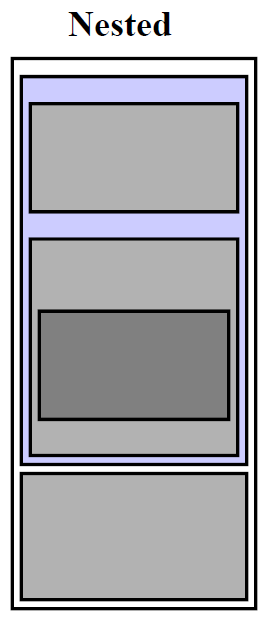
\includegraphics[scale=1]{rapport/2/figures/nested_block_structure}
		\end{center}	
		\caption{Illustration of the nested block structure }
	\end{wrapfigure}
	
	
	
	
	
	
	
	
	
	
%Page 142 i Brown!! :D